\let\negmedspace\undefined
\let\negthickspace\undefined
\documentclass[journal]{IEEEtran}
\usepackage[a5paper, margin=10mm, onecolumn]{geometry}
\usepackage{tfrupee}

\setlength{\headheight}{1cm}
\setlength{\headsep}{0mm}

\usepackage{gvv-book}
\usepackage{gvv}
\usepackage{cite}
\usepackage{amsmath,amssymb,amsfonts,amsthm}
\usepackage{algorithmic}
\usepackage{graphicx}
\usepackage{textcomp}
\usepackage{xcolor}
\usepackage{txfonts}
\usepackage{enumitem}
\usepackage{mathtools}
\usepackage{gensymb}
\usepackage{comment}
\usepackage[breaklinks=true]{hyperref}
\usepackage{tkz-euclide}

\graphicspath{{./figs/}}

\begin{document}
\title{4.8.6}
\author{AI25BTECH11010 - Dhanush Kumar}
\maketitle
\renewcommand{\thefigure}{\theenumi}
\renewcommand{\thetable}{\theenumi}

\noindent\textbf{Question:}
Find the coordinates of the foot of the perpendicular $\vec{Q}$ drawn from $P(3,2,1)$ to the
plane $2x - y + z + 1 = 0$. Also find the distance $\vec{P}\vec{Q}$ and the image of the point $\vec{P}$
treating this plane as a mirror.
\medskip

\noindent\textbf{Solution:}

The point and the plane normal are
\begin{align}
\vec{P} &= \myvec{3\\2\\1}, & \vec{n} &= \myvec{2\\-1\\1},
\end{align}

\begin{align}
\vec{n}^T\vec{x} = -1.
\end{align}

Let $\vec{Q}$ be the foot of the perpendicular from $\vec{P}$ to the plane and let $\lambda$ be the scalar such that
\begin{align}
\vec{P}-\vec{Q} &= \lambda\vec{n}\\
\vec{n}^T\vec{Q} &= -1. 
\end{align}
 we have $\vec{Q}=\vec{P}-\lambda\vec{n}$.
 Therefore,
\begin{align}
\vec{n}^T(\vec{P}-\lambda\vec{n}) &= -1 \\
\vec{n}^T\vec{P} - \lambda\|\vec{n}\|^2 &= -1.
\end{align}
Thus
\begin{align}
5 - 6\lambda &= -1 \quad\Rightarrow\quad \lambda = -1.
\end{align}
Therefore
\begin{align}
\vec{Q} &= \vec{P}-\lambda\vec{n} = \myvec{3\\2\\1} - (-1)\myvec{2\\-1\\1}
= \myvec{1\\3\\0}.
\end{align}

Distance:
\begin{align}
PQ = \|\vec{P}-\vec{Q}\| = \|\lambda\vec{n}\| = |\lambda|\|\vec{n}\| = 1\cdot\sqrt{6}=\sqrt{6}.
\end{align}

Image of $\vec{P}$ in the plane (reflection) is
\begin{align}
\vec{R} &= 2\vec{Q} - \vec{P} = 2\myvec{1\\3\\0} - \myvec{3\\2\\1} = \myvec{-1\\4\\-1}.
\end{align}

\bigskip
\noindent\textbf{Answer:} \(
\vec{Q}=(1,3,0),\; PQ=\sqrt{6},\; \vec{R}=(-1,4,-1).
\)
\begin{figure}[h!]
  \centering
   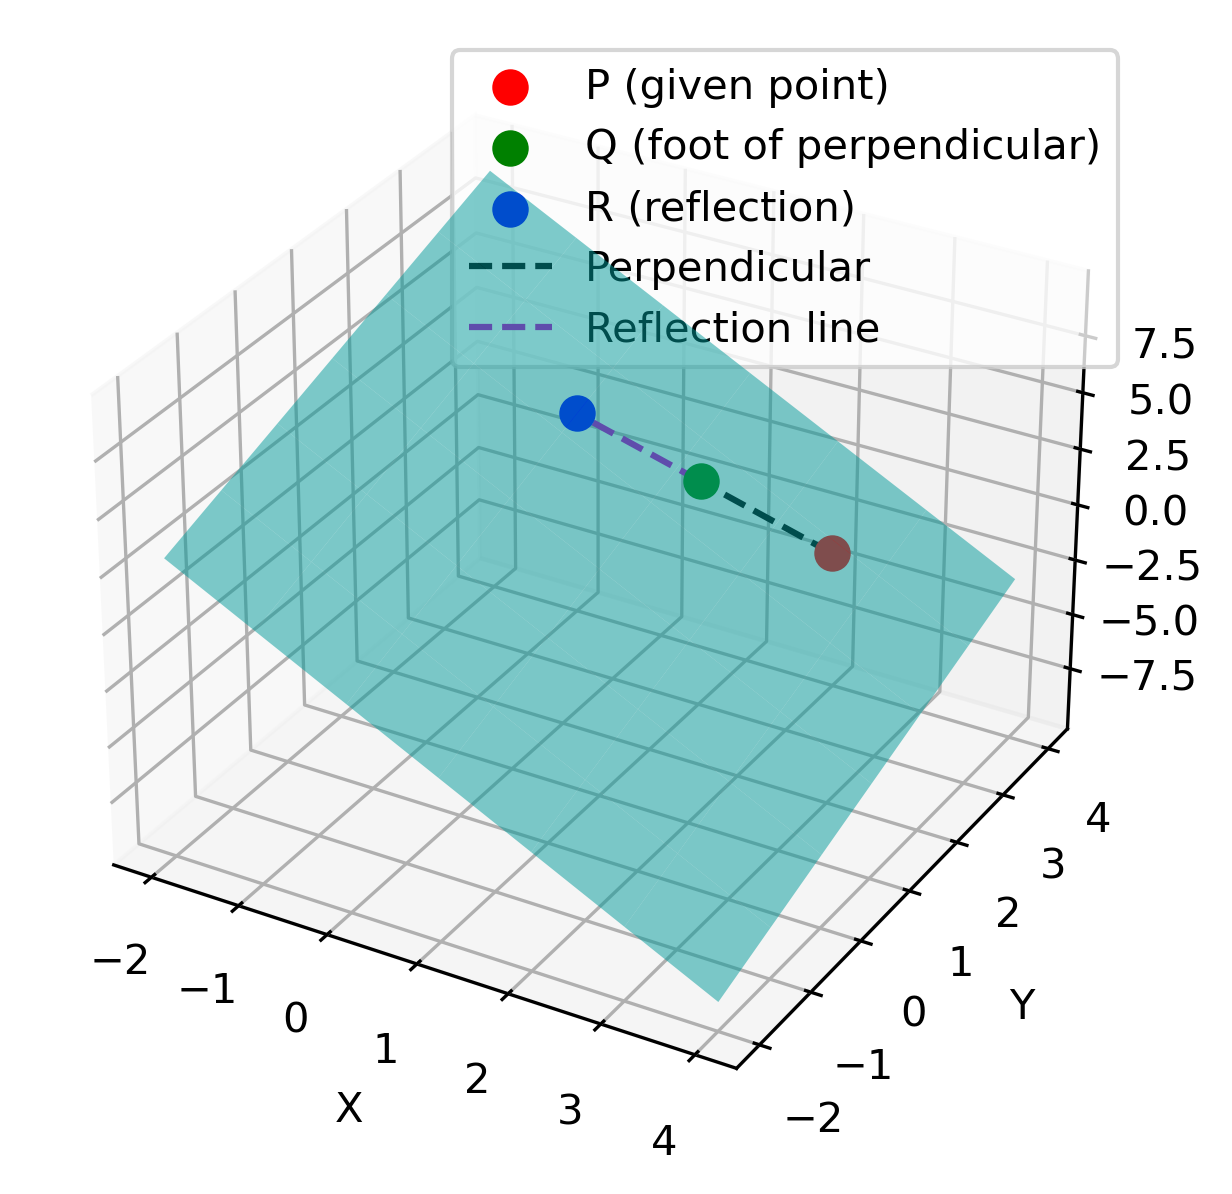
\includegraphics[width=0.7\linewidth]{../figs/point_plane.png}
   \caption{}
  \label{stemplot}
\end{figure}

\end{document}

